\documentclass[a4paper,twoside]{article}

\usepackage{epsfig}
\usepackage{subcaption}
\usepackage{calc}
\usepackage{amssymb}
\usepackage{amstext}
\usepackage{amsmath}
\usepackage{amsthm}
\usepackage{multicol}
\usepackage{pslatex}
\usepackage{apalike}
\usepackage{algorithm2e}
\usepackage[bottom]{footmisc}
\usepackage{booktabs}
\usepackage{graphicx}
\usepackage{url}
\usepackage{SCITEPRESS}

\newtheorem{proposition}{Proposition}
\graphicspath{{artifacts/}}

\begin{document}

\title{Does Looking at the Query Help: An Audit Protocol for LLM Routers}

\author{\authorname{Anonymous Author(s)}
\affiliation{Affiliation withheld for double-blind review}
\email{withheld@example.com}
}

\keywords{Large Language Models, Evaluation, Model Routing, Cost Accounting, Negative Results.}

\abstract{Query-conditioned routers assign each prompt to a cheap or an expensive language model and are routinely scored against always-frontier serving. That comparison is the wrong bar: a query-independent policy at the same expected dollar cost is the policy a router must beat to earn its complexity. This paper states an audit protocol---static and cost-matched mixture baselines, pre-registered one-shot tests, exact rather than mix-times-mean cost, and a decomposition of temperature-zero regeneration noise---and applies it to two systems. A deployed three-tier keyword router on 364 objectively graded items is dominated by always sending every query to the middle tier ($86.8\%$ at \$0.2867 versus $92.3\%$ at \$0.0418; McNemar exact $p=0.0003249$, Holm $p=0.0013$). That domination holds in $10{,}000/10{,}000$ item bootstraps and in every mix-simplex cell; the paired quality gap is HumanEval-driven. RouteLLM on its own GSM8K release ($n=1307$) beats a cost-matched mixture by a mean of $+0.57$ percentage points, with $0/9$ operating points significant. The protocol therefore separates a router that does not earn looking at the query from one that does, barely, at an effect size current benchmarks cannot resolve pointwise.}

\onecolumn \maketitle \normalsize \setcounter{footnote}{0} \vfill

\section{\uppercase{Introduction}}
\label{sec:introduction}

Large language model (LLM) serving is now routinely treated as a \emph{decision procedure}: given a query, choose a model, spend tokens, and return a graded answer. Routing papers report that this decision saves money relative to always calling a frontier model~\cite{chen2023frugalgpt,ong2025routellm,ding2024hybridllm}. The comparison is almost always the same. Traffic that would have gone to GPT-class models~\cite{openai2023gpt4} is diverted to smaller open models; the diverted fraction is multiplied by a published price; and the product is advertised as cost reduction, sometimes ``up to $85\%$.''

That headline answers a question nobody needed a classifier to ask. Always using the small model, or always using a competent mid-size model, also beats always-frontier on dollars. Neither policy reads the query. A router earns the machinery of looking at the query only if it beats a \emph{query-independent} policy that spends the same money. The right baseline is therefore not the frontier. It is the static assignment, or the random mixture, whose expected cost matches the router.

There is a second, quieter error. The cost axis itself is usually a mix-times-mean: the fraction of calls sent to each model, times that model's mean cost. For a query-independent policy the identity is exact, because assignment is independent of the item. For a real router it is biased. Routers escalate the items that generate more tokens. Substituting the unconditional mean therefore undercharges the router and overstates savings. The bias is not a modelling choice; it is the covariance between the routing indicator and per-item cost, and it has a closed form (Section~\ref{sec:accounting}).

This paper treats those two mistakes as an evaluation problem, not as an argument that routing is impossible. The contribution is an \emph{audit protocol} that a routing paper can run on its own artifacts, together with two applications that come out differently. The first system is a deployed three-tier keyword router (hereafter EcoLogic) on a frozen panel of $364$ objectively graded items: HumanEval~\cite{chen2021humaneval}, MMLU~\cite{hendrycks2021mmlu}, and GSM8K~\cite{cobbe2021gsm8k}. Cost is measured dollars from provider \texttt{usage} fields. Always-Tier-2, which ignores the query, is both more accurate and cheaper. That evaluation is in-sample for the keyword lists; the caption of Table~\ref{tab:stage12} says so. The second system is RouteLLM~\cite{ong2025routellm} scored on the authors' own released GSM8K responses, checkpoint, decontamination list, and threshold grid ($n=1307$). Against a cost-matched mixture the router wins on average by $+0.57$ percentage points. The direction is consistent ($8$ of $9$ interior operating points) and a sign test across the sweep reaches $p=0.039$, but \emph{no individual point} is significant at $p<0.05$. Matching on call fraction, the literature's usual proxy, overstates the edge by $0.09$--$0.30$ points.

A pre-registered learned replacement for EcoLogic, evaluated once on a held-out split, does not rescue the first system: the selected logistic router is numerically identical to always-cheap and to the cost-matched static policy (quality $0.8889$). Stronger learners on the same representation do not raise held-out discrimination above logistic calibration AUC $0.6816$. Temperature $0$ is not determinism: Tier~1 flips its graded verdict on $19.8\%$ of items across three regenerations, and $47\%$ of that tier's confidence-interval width is regeneration noise that more benchmark items would not remove.

The claim is therefore not ``routing does not work.'' It is that current reporting practice cannot tell a router that earns looking at the query from one that does not, because it uses the wrong baseline and a biased cost axis, and because the honest effect, when it exists, sits at or below the resolution of the benchmarks the field uses.

\noindent ICAART solicits completed work on Large Language Models, agent architectures, and evaluation of AI decision procedures. A query-conditioned router is such a procedure: it maps an observation (the prompt) to an action (which model to call). The paper's contribution is not a new agent, but a test of whether that mapping earns its complexity.

\noindent\textbf{Contributions.}
(1)~An audit protocol that any cross-API router evaluation can run on stored artifacts (Section~\ref{sec:protocol}, Table~\ref{tab:checklist}).
(2)~A closed-form identity showing that mix-times-mean cost is biased exactly by a covariance term, with a sign flip on both systems (Section~\ref{sec:accounting}).
(3)~A paired, in-sample audit of a deployed keyword router on measured USD (Study~A) and a reconstruction of RouteLLM on its own GSM8K release (Study~B).
(4)~A pre-registered held-out null, a MiniLM predictability ceiling, and a temperature-zero regeneration decomposition (Study~C).
All digits reconstruct from committed files via \texttt{papers/icaart/analysis.py}. No new model calls were made.

\section{\uppercase{Related Work}}

\paragraph{Query-conditioned routers.}
RouteLLM learns a binary (or ternary) preference router from human and synthetic pairwise data and reports quality as a function of the fraction of queries sent to the strong model~\cite{ong2025routellm}. The public evaluation code does not mention tokens or dollars; the README conversion of call fraction into ``up to $85\%$ cost reduction'' assumes a constant price per call within each model. HybridLLM~\cite{ding2024hybridllm}, AutoMix~\cite{aggarwal2024automix}, Tryage~\cite{hari2023tryage}, RouterDC~\cite{hu2024routerdc}, GraphRouter~\cite{feng2024graphrouter}, and TensorOpera Router~\cite{stripelis2024tensoropera} likewise treat routing as a learned assignment from prompt features to a model index. Shnitzer et al. study routing with benchmark datasets as the supervision source~\cite{shnitzer2023routing}. The evaluation pattern is stable across this family: a learned score, a threshold sweep, a plot against strong-model call fraction, and a qualitative claim that quality is ``close to GPT-4'' at a fraction of the calls. What varies is the featuriser (BERT, embeddings, graph encoders, length) and the supervision (preferences, benchmark correctness, dual contrastive losses). What does not vary is the absence of a cost-matched query-independent mixture and of per-item token traces in the public artifacts.

\paragraph{Mixtures of experts, Mixtral, and serving routers.}
Surveys of mixture-of-experts architectures~\cite{yue2024mixtralstyle} sit adjacent: those systems route \emph{inside} a single trained network~\cite{shazeer2017moe,fedus2022switch,jiang2024mixtral}, whereas the systems audited here choose among separately served models. Mixtral-style sparse gating is an existence proof that query-conditioned computation can work when the gate is trained jointly with the experts and the cost of a bad gate is a wasted expert, not a billed API call. Cross-API routers do not get that joint training. Treating a Mixtral gating paper as evidence that a keyword or BERT router over black-box endpoints will beat Always-Tier-2 is a category error, but it is a common one in related-work paragraphs. The audit protocol is designed for the cross-API case, where looking at the query has to pay for itself in graded accuracy at matched dollars.

\paragraph{Cascades and FrugalGPT.}
FrugalGPT~\cite{chen2023frugalgpt} cascades models in increasing order of cost and stops when a reliability estimator accepts the answer. Cascade cost is the sum of all attempts up to acceptance, so per-item cost varies with both response length and cascade depth. The authors report aggregate reductions against published list prices; there is no official per-query cost trace. Subsequent work on compound inference systems studies how quality scales with the number of LLM calls~\cite{chen2024cascade}. Meta-learning approaches such as Fly-Swat or Cannon~\cite{sakota2024fly} select a model per query from a cost--quality menu. All of these papers need a query-independent cost-matched baseline in order to isolate the value of reading the query. Few report one.

\paragraph{What is missing from the evaluation literature.}
Three gaps recur. First, always-frontier is the default comparator even when a cheaper static model already matches quality. Second, call fraction is treated as interchangeable with cost. Third, negative or null routing results are rare in print, which is a publication-filter problem rather than evidence that the null is false~\cite{gelman2013garden,nosek2018prereg}. The present paper is an evaluation-methodology contribution carried by two outcomes, one negative and one barely positive, obtained under a protocol that was written down before the held-out numbers existed.

\section{\uppercase{Audit Protocol}}
\label{sec:protocol}

The protocol has five pieces. None requires a new model.

\begin{algorithm}[t]
\DontPrintSemicolon
\caption{Audit a $k$-model cross-API router on a frozen panel.}
\label{alg:audit}
\KwIn{items $X$; generations and costs $c_j(x)$ for each model $j$; router $\hat t$; frozen test rule}
\KwOut{pass or fail, with McNemar and exact cost}
evaluate always-$j$ on the same generations, all $j$\;
$\pi \leftarrow n^{-1}\sum_i c_{\hat t(x_i)}(x_i)$ \tcp*{exact, not mix$\times$mean}
solve the cost-matched mixture $\alpha$ in~\eqref{eq:costmatch}\;
McNemar-exact $(\hat t$, always-$j^\star)$ and versus the mixture\;
Holm-adjust the family of paired tests\;
\eIf{$\hat t$ is less accurate or more expensive than the cost-matched policy}{\textbf{fail}: looking at the query did not earn its complexity}{\textbf{pass} only if the edge exceeds the panel's Monte Carlo SE}
\end{algorithm}

\subsection{Static single-tier baselines}

On a shared item set, evaluate always-model-$j$ for every $j$ in the menu, using the same generations the router is scored on. A router that loses to a constant on accuracy, or that wins on accuracy only by spending more than the constant, has not earned looking at the query. Oracle (cheapest correct model per item, hindsight) is reported as a headroom diagnostic, never as a deployable policy.

\subsection{Cost-matched query-independent mixtures}

For a two-model menu with per-item costs $c_w(x)$ and $c_s(x)$, let $\pi$ be the router's realised mean cost. The cost-matched mixture is the query-independent Bernoulli that uses the strong model with probability $\alpha$ solving
\begin{equation}
\alpha\,\mathbb{E}[c_s(X)] + (1-\alpha)\,\mathbb{E}[c_w(X)] = \pi,
\label{eq:costmatch}
\end{equation}
clipped to $[0,1]$. Its expected accuracy is $\alpha p_s + (1-\alpha)p_w$. Matching instead on the \emph{call} fraction $\hat\alpha = n^{-1}\sum_i 1\{\hat t_i = s\}$ is a different experiment: it ignores within-model cost dispersion. Section~\ref{sec:studyB} shows that the two matchings differ by $0.09$--$0.30$ percentage points on RouteLLM GSM8K. When the cheap model Pareto-dominates the menu, Equation~\eqref{eq:costmatch} collapses to always-cheap; that collapse is a finding about the price vector, not a bug in the protocol.

\subsection{Exact cost, not mix times mean}

Report realised per-item cost $\sum_i c_{\hat t(x_i)}(x_i)$. The mix-times-mean estimator is reserved for query-independent policies, where it is exact, or is accompanied by the covariance correction of Section~\ref{sec:accounting}.

\subsection{Pre-registration and one-shot frozen tests}

Success criteria, threshold-selection rules, and the identity of the frozen test set are committed before labels on that set are inspected~\cite{nosek2018prereg}. The EcoLogic learned-router addendum required either a McNemar exact improvement over Always-Tier-2 at $p<0.05$ (S1) or matched accuracy at $\ge 15\%$ lower energy (S2); neither was met. A later held-out protocol froze a $60/20/20$ split, fit features on train only, selected on validation only, and scored test once. Shopping among unselected rows after seeing test is not part of the protocol.

\begin{table}[t]
\centering
\caption{Minimum reportable set for a cross-API LLM router. Items 1--4 isolate the value of looking at the query; 5--6 bound statistical overclaim.}
\label{tab:checklist}
\scriptsize
\begin{tabular}{@{}p{0.22\columnwidth} p{0.68\columnwidth}@{}}
\toprule
Item & Requirement \\
\midrule
Static pool & Always-model-$j$ for every $j$, same generations. \\
Cost-matched mix & Query-independent Bernoulli at the router's realised mean USD, not at its call fraction. \\
Exact cost & $\sum_i c_{\hat t(x_i)}(x_i)$; mix$\times$mean only with the covariance correction. \\
One-shot test & Frozen split and selection rule committed before test labels. \\
Paired test & McNemar on identical items; Wilson intervals; no unpaired $t$ on accuracies. \\
Resolution & State whether the honest edge is smaller than the panel's Monte Carlo SE. \\
\bottomrule
\end{tabular}
\end{table}

\subsection{Paired tests and interval semantics}

Accuracy uses Wilson score intervals~\cite{wilson1927,newcombe1998}. Paired comparisons on identical items use McNemar's exact test (two-sided binomial on discordant pairs;~cite{mcnemar1947}). Unpaired $t$-tests on accuracies are not used. Operating-point sweeps share items; a sign test across a sweep~\cite{conover1980sign} is a descriptive consistency check, not an exact independent test, and is labelled as such. Temperature-zero regeneration is measured, not assumed away (Section~\ref{sec:studyC}).

\section{\uppercase{Cost-Accounting Bias}}
\label{sec:accounting}

Let $X$ be drawn from the evaluation distribution. For each model $j$ let $c_j(X)$ be the actual cost of $j$'s response to $X$, and write $c_j := \mathbb{E}[c_j(X)]$. Let $t^\star(X)$ be a reference assignment (oracle or any other) and $\hat t(X)$ the router's assignment. Write $C_{ij} := \{t^\star = i,\ \hat t = j\}$ and $D_{ij}(X) := c_j(X) - c_i(X)$. Define
\begin{align}
R_{\mathrm{true}} &= \mathbb{E}\bigl[c_{\hat t(X)}(X) - c_{t^\star(X)}(X)\bigr], \label{eq:rtrue}\\
R_{\mathrm{naive}} &= \sum_{i \neq j} \Pr(C_{ij})\,(c_j - c_i). \label{eq:rnaive}
\end{align}
$R_{\mathrm{naive}}$ is the confusion-matrix formula: cell probability times the difference of \emph{unconditional} model means.

\begin{proposition}
\label{prop:identity}
For any joint distribution of $(X,t^\star,\hat t)$ with finite first moments,
\[
R_{\mathrm{true}} = R_{\mathrm{naive}} + \sum_{i\neq j} \mathrm{Cov}\bigl(1_{C_{ij}},\, D_{ij}(X)\bigr).
\]
Hence $R_{\mathrm{naive}}=R_{\mathrm{true}}$ if and only if the sum of covariances vanishes. A sufficient condition is $\mathbb{E}[D_{ij}\mid C_{ij}]=\mathbb{E}[D_{ij}]$ for each off-diagonal cell; in particular the naive formula is exact when $c_j(X)$ is constant within each model.
\end{proposition}

\begin{proof}[Proof sketch]
Partition on the cells. Diagonal terms vanish because $D_{ii}=0$ pointwise, so
$R_{\mathrm{true}} = \sum_{i\neq j}\Pr(C_{ij})\,\mathbb{E}[D_{ij}\mid C_{ij}]$.
Subtracting~\eqref{eq:rnaive} termwise yields
$\sum_{i\neq j}\Pr(C_{ij})\bigl(\mathbb{E}[D_{ij}\mid C_{ij}]-\mathbb{E}[D_{ij}]\bigr)$.
For an event $A$ and integrable $D$, $\mathrm{Cov}(1_A,D)=\Pr(A)(\mathbb{E}[D\mid A]-\mathbb{E}[D])$. Applying this with $A=C_{ij}$ and $D=D_{ij}$ gives the claim.
\end{proof}

The algebra is the definition of covariance. It is load-bearing because the naive formula is how routing papers turn a call mix into a dollar figure. The sufficient condition---constant cost within a model---fails as soon as completion length varies. It fails in the router's favour: short, easy items go to the cheap model, so residual traffic on the expensive model is longer than that model's average item.

\paragraph{Numerical reconciliation.}
On the EcoLogic calibration split used to derive the identity ($n=360$), $R_{\mathrm{naive}}=-0.2496$ while $R_{\mathrm{true}}=+0.2840$ in the original per-item cost units of that derivation. The correction term is $+0.5336$, $1.88\times$ the size of true regret, and the two estimators disagree in sign. Adding the correction recovers $R_{\mathrm{true}}$ with residual $2.2\times 10^{-16}$. On the Stage~1--2 measured-USD panel, mix-times-mean understates EcoLogic's realised cost of \$0.2867 by \$0.0199 ($6.95\%$); the covariance identity reconciles with residual $1.1\times 10^{-19}$. For a static Always-Tier-2 assignment the same identity is exact up to floating point, as Proposition~\ref{prop:identity} requires.

On RouteLLM GSM8K (Section~\ref{sec:studyB}), naive accounting understates true cost at every non-degenerate operating point, by up to $6.3\%$, and flips the sign of oracle-regret at the $30\%$-strong threshold. Within-model cost coefficients of variation are $0.36$ (Mixtral) and $0.43$ (GPT-4). Those CVs are modest by 2026 reasoning-model standards; the correction scales with within-model dispersion, so the bias grows as menus include long thinking traces.

The practical instruction is trivial and almost never followed: store per-item prompt and completion token counts next to the routing bit. Providers already return them.

\section{\uppercase{Study A: A Keyword Router on Measured Dollars}}
\label{sec:studyA}

\subsection{Setup}

EcoLogic is a deployed three-tier Q\&A router. Evaluation substitutes were used because the original Together AI slugs were retired: Tier~1 is \texttt{Qwen/Qwen3.5-9B}, Tier~2 is \texttt{openai/gpt-oss-20b}, Tier~3 is \texttt{gpt-4o}. The frozen panel has $364$ items (HumanEval $164$, MMLU $100$, GSM8K $100$), graded by execution, letter match, and final-answer match respectively---no LLM-as-judge. Each item was completed by all three tiers. The production classifier \texttt{classify\_prompt\_local\_nlp} assigned a tier from the raw user query. Cost is the sum of provider \texttt{usd} fields. Wilson intervals and McNemar tests are computed on the same $364$ paired outcomes.

This comparison is \emph{in-sample} for the keyword heuristic: keyword lists and thresholds were not locked on a held-out split of this panel. The router does not read evaluation labels at decision time; that is a narrower statement than ``no leakage.'' Held-out evidence is in Section~\ref{sec:studyC}.

\subsection{Results}

Table~\ref{tab:stage12} is the audit. Always-Tier-2 attains $336/364$ ($92.3\%$, Wilson $[89.1\%, 94.6\%]$) at \$0.0418. EcoLogic attains $316/364$ ($86.8\%$, $[82.9\%, 89.9\%]$) at \$0.2867. The accuracy gap is $+5.5$ percentage points for the constant policy. McNemar's exact test on discordant pairs $(b,c)=(5,25)$ gives $p=0.0003249$: on $25$ items Tier~2 is right where EcoLogic is wrong, and the reverse occurs on $5$. EcoLogic is also more expensive by a factor of $6.87$. Always-Tier-1 is statistically indistinguishable from EcoLogic on accuracy (McNemar $p=0.25$) and still more expensive. Random assignment, which ignores difficulty but not the existence of the two stronger tiers, scores $90.7\%$ at \$0.3628 (McNemar $p=0.0066$). Always-frontier is $91.5\%$ at \$0.6366 (McNemar $p=0.0095$). The hindsight oracle reaches $96.4\%$ at \$0.0470, locating headroom that the keyword policy does not capture.

On this price vector Tier~2 Pareto-dominates Tiers~1 and~3 on the panel means, so the cost-matched static mixture \emph{is} Always-Tier-2. The protocol does not have to invent a fractional mix. The router loses to the unique query-independent policy at its own cost scale, and also loses at the cheaper Always-Tier-2 scale.

The mechanism is visible in the mix: $274/87/3$ items go to Tiers~1/2/3. Escalations away from Tier~1 do not systematically rescue items Tier~1 got wrong. A router that concentrates traffic on the weakest expensive model, while a cheaper mid-size model is both more accurate and an order of magnitude cheaper per item, has not justified a query-conditioned policy.

Per-benchmark accuracies on the same generations explain why the constant is so strong. Across all $364$ items the three tiers score $87.6\%$, $92.3\%$, and $91.5\%$ (Wilson intervals $[83.9,90.6]$, $[89.1,94.6]$, $[88.2,93.9]$). The spread is under five points. On GSM8K they are $95/94/95$ in $100$---indistinguishable. On HumanEval, Tier~2 leads ($96.3\%$) and Tier~3 is second ($91.5\%$); McNemar tests on the full panel find Tier~2 versus Tier~3 non-significant ($p=0.711$, discordant $16/13$). There is no paired quality justification for escalating from the middle tier to the frontier on this workload. Routing can only buy quality where models actually disagree, and on two of three benchmarks they barely do. The oracle row in Table~\ref{tab:stage12} still sits at $96.4\%$, because disagreements that do exist are not nested: an ideal assignment would beat every single model. The keyword policy captures none of that complementary error structure.

A secondary surface-form check, not used as a headline, shows that feeding the classifier the wrapped benchmark prompt rather than the raw query agrees on only $53.0\%$ of items and sends all $164$ HumanEval programs to Tier~3. All numbers in Table~\ref{tab:stage12} use the raw query, which is what a user types and which is the surface more favourable to the router. Choosing the wrapped surface after seeing both would be a researcher degree of freedom; both were computed, and the published surface is the production one.

\subsection{Robustness: mix, bootstrap, and the hindsight assignment}
\label{sec:robustA}

Three tests ask whether Table~\ref{tab:stage12} is an artifact of the $45/27/27$ HumanEval/MMLU/GSM8K mix or of a lucky draw of $364$ items.

Leave-one-benchmark-out and single-benchmark slices: Always-Tier-2 remains cheaper \emph{and} at least as accurate on all seven subsets (all, drop each benchmark, each benchmark alone). Cost domination is therefore not a mix accident. Quality domination \emph{is} concentrated: McNemar versus Always-T2 is $p=1.2\times 10^{-4}$ on HumanEval ($n=164$, discordant $2/20$) and is not significant on MMLU-only ($p=1$, $2/3$) or GSM8K-only ($p=1$, $1/2$). A reviewer who discards HumanEval still cannot save the router on dollars (\$0.139 vs.\ \$0.018 on the remaining $200$ items). We report that split rather than averaging it away.

A $21$-cell simplex of benchmark weights (step $0.2$) reweights per-benchmark mean USD. Always-T2 is cheaper than EcoLogic in $21/21$ cells. Item-resampling bootstrap ($10{,}000$ draws of the $364$ items): Always-T2 dominates on both accuracy and USD in $10{,}000/10{,}000$ draws. The $95\%$ bootstrap interval on the accuracy gap is $[+2.7,+8.5]$ points; on the USD gap, Always-T2 is cheaper by \$0.20--\$0.29. Cohen's $g$ on the full-panel McNemar is $0.33$ (a large paired effect). Holm adjustment of the five McNemar tests leaves Always-T2 at $p_{\mathrm{Holm}}=0.0013$. Dollar cost per correct answer is \$0.000907 (EcoLogic) versus \$0.000124 (Always-T2): a $7.3\times$ evaluation-unit gap that does not depend on calling Always-T2 the ``default.''

The keyword assignment agrees with the hindsight cheapest-correct oracle on only $89/364$ items ($24.5\%$). The mass of the disagreement is EcoLogic sending $257$ items to Tier~1 that the oracle would have sent to Tier~2. Looking at the query, on this classifier, is mostly a decision to avoid the model that the labels say is cheapest-and-correct. Fig.~\ref{fig:lob} shows the per-benchmark accuracy bars; Table~\ref{tab:lob} is the corresponding paired audit.

\begin{table}[t]
\centering
\caption{Study~A leave-one-benchmark-out. Always-T2 is cheaper on every slice. Quality McNemar is HumanEval-driven; dropping HumanEval leaves a dollar gap (\$0.139 vs.\ \$0.018) that the router still loses.}
\label{tab:lob}
\scriptsize
\begin{tabular}{@{}l r r r r r@{}}
\toprule
Subset & $n$ & Eco & T2 & Eco \$ & T2 \$ \\
\midrule
all & $364$ & $86.8\%$ & $92.3\%$ & $0.287$ & $0.042$ \\
drop HumanEval & $200$ & $88.0\%$ & $89.0\%$ & $0.139$ & $0.018$ \\
only HumanEval & $164$ & $85.4\%$ & $96.3\%$ & $0.147$ & $0.024$ \\
only MMLU & $100$ & $83\%$ & $84\%$ & $0.074$ & $0.007$ \\
only GSM8K & $100$ & $93\%$ & $94\%$ & $0.065$ & $0.011$ \\
\bottomrule
\end{tabular}
\end{table}

\begin{figure}[t]
\centering
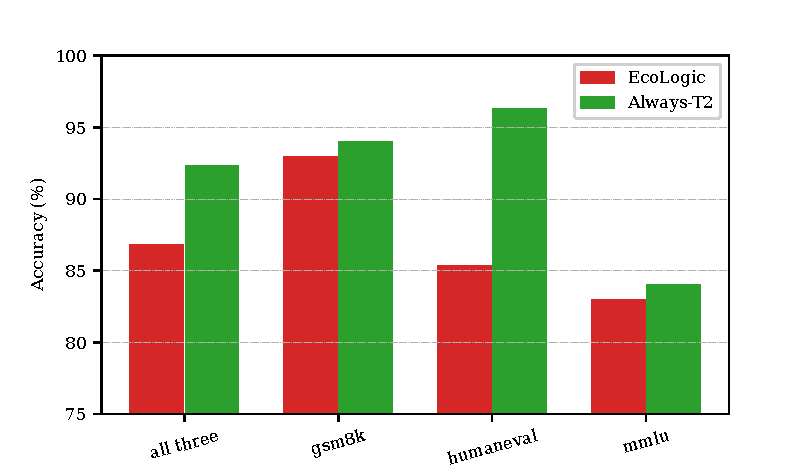
\includegraphics[width=\columnwidth]{fig_lob.pdf}
\caption{Study~A robustness: EcoLogic versus Always-T2 accuracy on the full panel and on each benchmark alone. Always-T2 is at least as accurate on every slice; the McNemar rejection lives in HumanEval.}
\label{fig:lob}
\end{figure}

\begin{table*}[t]
\centering
\caption{Study~A, measured USD, $n=364$ identical items. Accuracy intervals are $95\%$ Wilson score intervals. McNemar exact $p$-values are paired against EcoLogic; Holm-adjusted $p$ for Always-T2 is $0.0013$ (family of five tests). Discordant counts are (EcoLogic-only correct)\,/\,(other-only correct). \textbf{In-sample caveat:} the keyword classifier was not trained or thresholded on a held-out split of this panel. Oracle uses hindsight labels and is not a deployable policy. Random uses the stored seeded assignment.}
\label{tab:stage12}
\scriptsize
\begin{tabular}{@{}l r r r r r r@{}}
\toprule
Policy & Acc.\ $[95\%\ \mathrm{CI}]$ & USD & vs frontier & Mix T1/T2/T3 & McNemar $p$ \\
\midrule
EcoLogic (keyword, raw) & $86.8\%$ $[82.9,89.9]$ ($316/364$) & $0.2867$ & $0.450\times$ & $274/87/3$ & --- \\
Always Tier 1 & $87.6\%$ $[83.9,90.6]$ ($319/364$) & $0.3342$ & $0.525\times$ & $364/0/0$ & $0.25$ ($0/3$) \\
Always Tier 2 & $92.3\%$ $[89.1,94.6]$ ($336/364$) & $0.0418$ & $0.066\times$ & $0/364/0$ & $0.0003249$ ($5/25$) \\
Random tier & $90.7\%$ $[87.2,93.2]$ ($330/364$) & $0.3628$ & $0.570\times$ & $125/107/132$ & $0.006611$ ($5/19$) \\
Always-frontier (\texttt{gpt-4o}) & $91.5\%$ $[88.2,93.9]$ ($333/364$) & $0.6366$ & $1.000\times$ & $0/0/364$ & $0.009475$ ($11/28$) \\
Oracle (cheapest correct) & $96.4\%$ $[94.0,97.9]$ ($351/364$) & $0.0470$ & $0.074\times$ & $9/343/12$ & $5.821{\times}10^{-11}$ ($0/35$) \\
\bottomrule
\end{tabular}
\end{table*}

\begin{figure}[t]
\centering
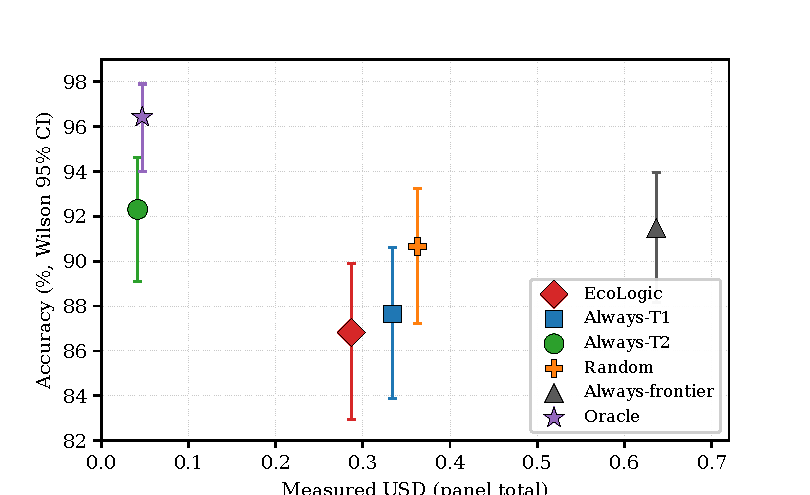
\includegraphics[width=\columnwidth]{fig_cost_accuracy.pdf}
\caption{Study~A: measured USD versus accuracy ($n=364$). Vertical bars are Wilson $95\%$ intervals. Always-Tier-2 (circle) Pareto-dominates EcoLogic (diamond) on both axes. In-sample keyword classifier.}
\label{fig:costacc}
\end{figure}

\section{\uppercase{Study B: RouteLLM on Its Own GSM8K Data}}
\label{sec:studyB}

Study~A could be a local failure of one keyword list. Study~B asks whether the same protocol, on someone else's router, someone else's models, and someone else's release, still changes the reported effect.

\subsection{What the release actually contains}

The RouteLLM repository (Ong et al., ICLR 2025; commit used for reconstruction documented with the artifacts) ships GSM8K response text for both Mixtral-8x7B-Instruct and GPT-4-1106-preview, plus correctness flags, a contamination list, and a BERT checkpoint. After their decontamination procedure, $n=1307$ of $1319$ rows remain. MMLU and MT-Bench in the same release do \emph{not} include response text, so per-item cost is not reconstructable there. The honest scope is one benchmark, one of five routers (the BERT router; matrix-factorisation and ranking routers need live embedding APIs and were not re-run), and one model pair.

Token counts are recovered by tokenizing released strings with \texttt{cl100k\_base} for GPT-4 and Mixtral's SentencePiece tokenizer for the weak model. Prices are contemporaneous list prices (\$ per 1M tokens): GPT-4-1106-preview $10.00$ in / $30.00$ out; Mixtral $0.60$ in / $0.60$ out. Absolute dollars therefore depend on a price vector this study supplies; the naive-versus-true \emph{gap} is driven by length covariance and is not an artifact of the overall price level. Mixtral accuracy is $63.73\%$; GPT-4 accuracy is $85.77\%$. Routing follows the authors' rule: softmax over the three-way head, win rate $1-(p_{\mathrm{tie}}+p_{\mathrm{weak}})$, thresholded on their \texttt{qcut} grid.

\subsection{Call-fraction matching is not cost matching}

Table~\ref{tab:routellm} reports the interior of the published threshold grid. At matched \emph{call} fraction---the quantity RouteLLM's evaluation actually plots---the mean router edge is $+0.76$ percentage points. At matched \emph{cost} (Equation~\eqref{eq:costmatch}) the mean edge is $+0.57$ percentage points. The difference, $0.09$--$0.30$ points depending on the operating point, is exactly the call-fraction proxy's overstatement. Eight of nine interior points still favour the router on the cost-matched axis; one (near $70\%$ strong) does not. Monte Carlo $p$-values against the cost-matched mixture are all $\ge 0.055$; \textbf{$0$ of $9$ points are significant at $p<0.05$}. A two-sided sign test on the nine cost-matched edges, treating the sign pattern as $8$ positive out of $9$, gives $p=0.0390625$. Operating points share items and are not independent, so this is a descriptive consistency check, not an exact test.

RouteLLM therefore \emph{passes} the audit in direction: looking at the query is better, on average, than a query-independent mixture at the same expected dollar cost. It passes narrowly. An effect of half a percentage point on $n=1307$ is smaller than the Monte Carlo standard deviation of the mixture at most thresholds (typically $0.5$--$0.8$ points). Headline ``up to $85\%$ cost reduction'' is a statement about call counts under a constant-price-per-call assumption. Under exact cost and a cost-matched baseline, the quality claim shrinks to $+0.57$ points and becomes undetectable threshold-by-threshold.

Implied Monte Carlo standard errors at the nine interior points have median $0.43$ percentage points. Detecting a $+0.57$ point mean edge at two-sided $\alpha=0.05$ with $80\%$ power would require $n\approx 5834$ independent GSM8K-like items---$4.5\times$ the released panel. Shared items across the sweep make that a lower bound. The field is therefore not under-powered for EcoLogic-scale failures (McNemar $p=3.2\times 10^{-4}$ on $n=364$); it is under-powered for RouteLLM-scale successes.

\begin{figure}[t]
\centering
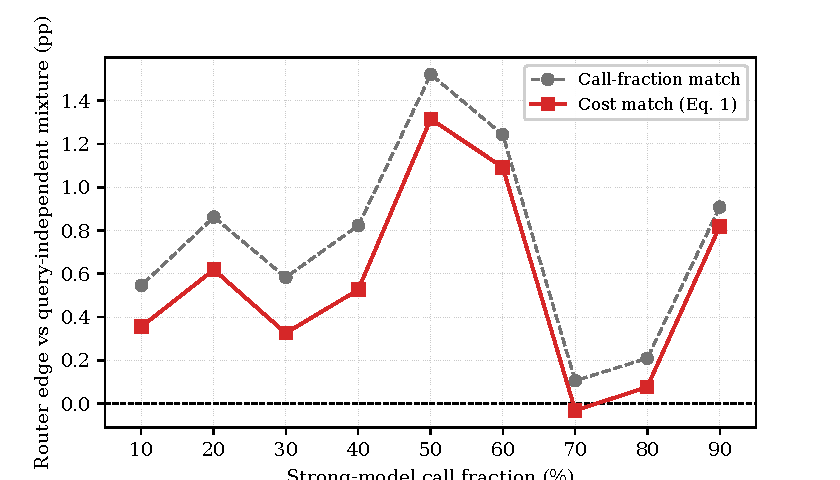
\includegraphics[width=\columnwidth]{fig_routellm_edge.pdf}
\caption{Study~B: RouteLLM BERT-router edge on released GSM8K ($n=1307$). Call-fraction matching (dashed) sits above cost matching (solid) at every interior threshold; both hover near the Monte Carlo noise floor. No interior $p<0.05$.}
\label{fig:rl}
\end{figure}

\begin{table*}[t]
\centering
\caption{Study~B: RouteLLM BERT router on released GSM8K ($n=1307$). Interior operating points of the authors' threshold grid. Edge is router accuracy minus the query-independent mixture, in percentage points. Call-fraction matching is the literature default; cost matching is Equation~\eqref{eq:costmatch}. Monte Carlo $p$ is versus the cost-matched mixture ($20{,}000$ draws). No interior $p$-value is below $0.05$.}
\label{tab:routellm}
\scriptsize
\begin{tabular}{@{}r r r r r r r@{}}
\toprule
Strong $\%$ & Router acc.\ $\%$ & Edge, frac.\ match (pp) & Edge, cost match (pp) & Lost to cost match (pp) & MC $p$ \\
\midrule
$90.0$ & $84.47$ & $+0.91$ & $+0.82$ & $0.09$ & $0.055$ \\
$80.0$ & $81.56$ & $+0.21$ & $+0.08$ & $0.13$ & $0.480$ \\
$70.0$ & $79.27$ & $+0.11$ & $-0.03$ & $0.14$ & $0.542$ \\
$60.0$ & $78.19$ & $+1.24$ & $+1.09$ & $0.15$ & $0.099$ \\
$50.0$ & $76.28$ & $+1.52$ & $+1.32$ & $0.21$ & $0.063$ \\
$40.0$ & $73.37$ & $+0.82$ & $+0.53$ & $0.30$ & $0.282$ \\
$30.0$ & $70.93$ & $+0.58$ & $+0.33$ & $0.26$ & $0.353$ \\
$20.0$ & $69.01$ & $+0.86$ & $+0.62$ & $0.24$ & $0.198$ \\
$10.0$ & $66.49$ & $+0.55$ & $+0.36$ & $0.19$ & $0.268$ \\
\midrule
Mean (interior) & --- & $+0.76$ & $+0.57$ & $0.09$--$0.30$ & $0/9$ sig. \\
\bottomrule
\end{tabular}
\end{table*}

\subsection{Accounting bias on the same sweep}

Applying Proposition~\ref{prop:identity} to the reconstructed per-item dollars, $R_{\mathrm{naive}}+{\mathrm{correction}}=R_{\mathrm{true}}$ at every threshold with maximum absolute residual $8.7\times 10^{-19}$. Naive cost is below true cost at every non-degenerate point. The largest relative gap is $6.31\%$ (at $10\%$ strong). At $30\%$ strong, naive oracle-regret is positive ($+3.21\times 10^{-5}$ \$/item) while true regret is negative ($-9.23\times 10^{-5}$): the same sign flip observed on EcoLogic, now on public data, in the region where a cost--quality paper is most likely to quote a single operating point.

This is not a refutation of RouteLLM's quality-versus-call-fraction curves. Those curves do not use Proposition~\ref{prop:identity}. It is a refutation of the silent step that turns the curves into a cost claim without a cost-matched query-independent baseline.

\section{\uppercase{Study C: Pre-registered Learning, a Predictability Ceiling, and Regeneration Noise}}
\label{sec:studyC}

Keyword failure might be an implementation complaint. Study~C replaces the heuristic under a protocol that forbids post-hoc rescue.

\subsection{Held-out learned replacement: a null}

A $1200$-item pool (MBPP~\cite{austin2021mbpp} substituting for HumanEval to avoid contaminating the frozen $164$, plus held-out MMLU and GSM8K) was split $720/237/243$ by a frozen manifest. TF-IDF and scalers were fit on train only. Thresholds and hyperparameters were selected on validation only. Candidates were logistic regression, a boosted tree, a length threshold, and the frozen production heuristic. The selection criterion, committed in advance, maximised validation quality advantage versus the in-sample cost-matched static hull.

Validation selected \textbf{logistic} with quality advantage $0.0$. On the untouched test split ($n=243$), logistic quality is $0.8889$ at \$0.0001526 per item---\emph{numerically identical} to \texttt{always\_cheap}, \texttt{random\_matched}, and \texttt{cost\_matched\_static}. The quality advantage versus cost-matched static is $0.0$; the paired $p$-value stored with the row is $1.0$. This is a null. It is not a successful learned router. The production heuristic on the same split scores $0.860$ at several times the dollar cost. The hindsight oracle reaches $0.942$, so the split is not saturated; the selected deployable method simply copies Always-Tier-2.

An earlier one-shot evaluation of a MiniLM~\cite{wang2020minilm,reimers2019minilm} logistic router on the original frozen $364$-item panel (pre-registered S1/S2; test scored once) produced $92.0\%$ versus Always-Tier-2's $92.3\%$, McNemar exact $p=1$ (discordant pair $(0,1)$). Neither S1 nor S2 was met. That comparison used a modelled energy constraint for S2; the present paper does not treat modelled energy as a measured result. The accuracy null is the part that transfers.

\subsection{Ceiling AUC}

If the null is ``we used a weak model class,'' stronger learners on the same representation should beat the linear head out of sample. Table~\ref{tab:ceiling} reports one-shot calibration AUCs on MiniLM embeddings (TRAIN $n=3500$, CALIBRATION $n=1500$; frozen test untouched). Logistic mean calibration AUC is $0.6816$. Gradient boosting, random forest, and $k$-NN ($k=50$) are all worse on calibration, despite random forest reaching TRAIN AUC $0.9999$. Ample capacity, zero held-out gain, is the signature of a weakly predictable label, not of an inadequate hypothesis class. A fine-tuned LLM router might extract more signal; that experiment was not run. The cheap explanation is ruled out.

\begin{table}[t]
\centering
\caption{Predictability ceiling on MiniLM features. Fit on TRAIN, scored once on CALIBRATION. Mean AUC averages the Tier~1 and Tier~2 heads.}
\label{tab:ceiling}
\scriptsize
\begin{tabular}{@{}l cc@{}}
\toprule
Model & Mean calib.\ AUC & Mean train AUC \\
\midrule
Logistic (router head) & $\mathbf{0.6816}$ & $0.8140$ \\
Gradient boosting & $0.6547$ & $0.9577$ \\
Random forest & $0.6703$ & $0.9999$ \\
$k$-NN ($k=50$) & $0.6521$ & $0.7835$ \\
\bottomrule
\end{tabular}
\end{table}

\subsection{Temperature zero is not deterministic}

The Stage~7 frozen set was regenerated $k=3$ times per item per tier at temperature $0$. A flip is an item whose graded verdict changes across those replicates. Tier~1 flips on $72/364$ items ($19.8\%$); mean within-item token standard deviation is $1936$ tokens. Tier~3 (\texttt{gpt-4o}) flips on $5/364$ ($1.4\%$). A variance decomposition of a single-draw accuracy splits Bernoulli variance into between-item and within-item (regeneration) components. For Always-Tier-1, regeneration is $47\%$ of the total; for Always-frontier it is $4.9\%$. Wilson intervals already include the single-draw noise, so they are not too narrow as coverage statements. They are easy to \emph{misread} as sampling-only uncertainty about a deterministic model. Comparisons whose margin sits inside the sampling-plus-generation half-width cannot be resolved by adding items unless the comparison is paired on identical generations---which is why every McNemar test in this paper is paired.

\section{\uppercase{Discussion}}

The protocol is not a machine for rejecting routers. It is a separator. Table~\ref{tab:verdict} records the three applications against the same five checks. EcoLogic fails on both axes at once, in-sample, on measured dollars, with a McNemar $p$-value three orders of magnitude below $0.05$. RouteLLM passes in sign and in a sweep-level sign test, and fails as a pointwise statistical claim. The held-out logistic copies Always-Tier-2. That triple is more informative than any one result. If every router failed, the protocol would be suspected of being stacked. If every router passed comfortably, the accounting correction would look pedantic. What the field actually has is a mixture of systems that do not earn their complexity and systems whose honest effect is smaller than a $1307$-item GSM8K panel can resolve at a single threshold.

\begin{table}[t]
\centering
\caption{Audit verdicts. Cost-matched is Equation~\eqref{eq:costmatch}; on Study~A it collapses to Always-Tier-2.}
\label{tab:verdict}
\scriptsize
\begin{tabular}{@{}llll@{}}
\toprule
Study & vs matched & $p{<}0.05$ & Verdict \\
\midrule
A keyword & worse, $6.87\times$ \$ & yes (vs router) & fail \\
B RouteLLM & ${+}0.57$\,pp mean & $0/9$ points & directional \\
C logistic & identical & $p{=}1$ & copies T2 \\
\bottomrule
\end{tabular}
\end{table}

Effect size versus benchmark resolution is the evaluation fact that routing papers currently bury. A mean edge of $+0.57$ points is a real directional signal and a rounding error on a camera-ready plot of ``GPT-4 quality at $20\%$ of the calls.'' Call-fraction matching adds another $0.09$--$0.30$ points of optical advantage. Mix-times-mean cost adds up to $6.3\%$ of further optimism on the dollar axis. Stacked on always-frontier as the only baseline, the visual impression is of a solved systems problem. Unstacked, the problem is still open, and some deployed classifiers are worse than ignoring the query.

A back-of-envelope for resolution is useful. A McNemar test on $n=1307$ with a $0.57$ point systematic edge, if discordant pairs were a few percent of items, is not guaranteed to reject at $\alpha=0.05$ at a single threshold; the Monte Carlo standard deviations in Table~\ref{tab:routellm} ($0.5$--$0.8$ points) already say as much. Temperature-zero flips of $19.8\%$ on long-output models imply that unpaired cross-paper comparisons of ``router A versus router B'' at the one-point scale are not even measuring the same random variable unless generations are cached. The protocol's pairing requirement is therefore not statistical pedantry. It is the difference between a number that can be reconstructed from a JSONL file and a number that moves when the endpoint is called again.

The held-out logistic identity with Always-Tier-2 is the honest continuation of Study~A. Once the price vector makes the middle tier both accurate and cheap, a well-regularised learner with weak prompt signal copies the constant. Reporting that copy as a ``learned router'' would be a success by redefinition. The protocol records the selected method and the identical metrics, and stops.

\section{\uppercase{Limitations}}

Hostile readings are anticipated here rather than in a rebuttal.

\paragraph{In-sample keyword evaluation.}
Table~\ref{tab:stage12} audits a production heuristic on the panel used to inspect it. Keyword lists were not cross-validated. The result is still a valid statement about that deployed classifier on those $364$ items; it is not a generalisation bound. The held-out protocol (Section~\ref{sec:studyC}) is the out-of-sample statement, and it is a null.

\paragraph{Substituted models.}
Tiers~1 and~2 are not the originally named production slugs. The routing \emph{logic} is what is tested. A different mid-size model could change Always-Tier-2's location on the hull. The protocol would still apply; the domination numbers would not automatically transfer.

\paragraph{One external benchmark.}
RouteLLM is checked on GSM8K only, because that is the only artifact with response text. Token counts are reconstructed, not billed. Prices are this study's input. The BERT router is one of five. FrugalGPT has no public per-query trace and was not estimated from aggregates.

\paragraph{Pool reuse.}
The $1200$-item held-out pool overlaps historically with earlier feature work. The new split is ID-disjoint internally; prior peeking at the pool is not fully controlled. Soft near-duplicates at Jaccard $0.7$--$0.9$ exist (exact and $\ge 0.9$ duplicates do not).

\paragraph{No joule meter, no latency claim.}
Energy was not physically measured. This paper's primary axis is provider USD and graded accuracy. Wall-clock serving latency is out of scope. No Cloud Run or Lambda measurement is claimed; committed deployment stubs are local dry-runs.

\paragraph{Menu geometry.}
On the Stage~1--2 price vector, Tier~2 dominates, so there is little room for a router to help. That is a property of this menu, not of routing as a concept. Menus whose quality strictly increases with cost have more headroom; they still require cost-matched baselines and exact cost.

\paragraph{Scope of the negative.}
One family of zero-API-cost routers, academic single-turn items, substituted tiers, and one public two-model router on one benchmark cannot support ``routing cannot work.'' RouteLLM and FrugalGPT report gains in their own settings. The present claim is about how those gains are measured.

\section{\uppercase{Conclusion}}

Looking at the query is a hypothesis about a decision procedure, and hypotheses need the right control. The control is a query-independent policy at the same expected cost, scored with realised per-item dollars, on a frozen test that was not used to tune the decision. Under that protocol a deployed keyword router is strictly worse than a constant, a pre-registered learned replacement copies the constant, and a published learned router improves GSM8K by half a point---detectable as a sign pattern, not as a per-threshold significance test. The mix-times-mean cost formula that converts those results into savings is biased by a covariance term that can flip signs and that overstates RouteLLM savings by up to $6.3\%$. Evaluation practice, not architecture, is the bottleneck. Routing papers can close it by publishing per-item tokens, a cost-matched mixture, a McNemar test, and a sentence that states whether looking at the query beat not looking.

\section*{Acknowledgements}

Omitted for double-blind review.

\bibliographystyle{apalike}
\bibliography{refs}

\end{document}
